\chapter{Introduction} \label{chap:introduction}

Medical diagnosis and specifically computer-aided diagnosis (CAD) is a hot topic in the field of technology. One of the main reasons for becoming a hot topic is the recent innovation and breakthroughs achieved by computer vision research. Combined with poor healthcare coverage around the globe, CAD systems offer a promising solution to mitigate the devastating impact of fatal diseases such as pneumonia. Controversial topics such as whether or not artificial intelligence will replace the radiologist in the future aside, these automated systems can offer answers for patient's questions in absence of medical help or to very least offer much needed second opinion in the face of unsatisfied diagnoses. Given all the mentioned possible benefits of the CAD systems, this project is focused on building classification CAD systems for diagnosing pneumonia from the chest X-ray images.

\section{Aims and Objectives} \label{sec:aimsandobj}
The aim of this project is to build a fully functional chest X-ray image classification pipeline that implements CI/CD principals to experimentation and deployment.

\subsection{Objectives}
Project will be implemented with execution of fallowing objectives:
\begin{enumerate}
    \item \textbf{Carrying out general data exploration: }This part involves general check on dataset.
    \item \textbf{Data pre-processing and augmentation: }Preparing the data for model ready state.
    \item \textbf{Building baseline model with well known neural network architectures: }This step involves setting additional benchmarks with out of the box models from section 4.
    \item \textbf{Using pre-trained network to increase model performance: }Using pre-trained networks to help training and accuracy of the model.
    %\item Model improvement and hyper parameter tuning
    \item \textbf{Visualizing neural network to ensure learning quality: } For making sure model learning as intended and focusing on correct parts of the image.
    \item \textbf{Model ensembling: }Using ensemble method with different neural network architectures.
    %\item \textbf{Model refinement: } Prototyping for improved model thorough hyper-parameter tuning.
    %\item Saving trained model for deployment
    \item \textbf{Applying different deployment options: } Implementation of different deployment options. Based on their trade offs. 
\end{enumerate}
It's worth emphasizing that the objective of this project is not to achieve the state of the art result in pneumonia detection but to offers a preferred method for improving and enhancing the existing models.
The intuition behind choosing the above objectives instead of attempting to build novel architecture from scratch is the process of choosing a novel architecture has a very large search space and requires a lot of iteration and experimentation. Due to the limited time frame of this project attempting to find new architecture would not be feasible. Additionally, objectives designed to serve the project goal with consistent aims. For example, item 1 and 2 will focus on reducing the model over-fitting while item 5 would serve as a tool to detect over-fitting. Objective 2 serves as a selection for a suitable model and setting benchmark while 6 is aimed at improving the model.

\section{CI/CD Pipeline} \label{sec:cicd}
In this section, I will give a brief introduction to the CI/CD pipeline to explain what CI/CD is and why it is chosen as a preferred way to build this project.

Continuous integration (CI) is a workflow strategy that helps ensure everyone's changes will integrate with the current version of the project in the typical software engineering team. This lets members of the team catch bugs, reduce merge conflicts, and increase overall confidence that your software is working. While the details may vary depending on the development environment, most CI systems feature the same basic tools and processes. In most scenarios, a team will practice CI in conjunction with automated testing using a dedicated server or CI service. Whenever a developer adds new work to a branch, the server will automatically build and test the code to determine whether it works and can be integrated with the code on the main development branch. The CI server will produce output containing the results of the build and an indication of whether or not the branch passes all the requirements for integration into the main development branch. By exposing build and test information for every commit on every branch, CI paves the way for what's known as continuous delivery, or CD, as well as a related process, called continuous deployment. The difference between continuous delivery and continuous deployment is that CD is the practice of developing software in such a way that you could release it at any time. When coupled with CI, continuous delivery lets you develop features with modular code in more manageable increments. Continuous development is an extension of continuous delivery. It's a process that allows you to actually deploy newly developed features into production with confidence, and experience little if any, downtime. Even though the benefits of using CI/CD pipelines are more prominent in the software teams, integration automated testing will help even individual projects such as this by reducing time for debugging.

In more granular detail, this system works with central version control services and in this project central version control service used is Github. GitHub uses a communication tool called \emph{webhooks} to send messages to external systems about activities and events that occurred in the project. For each event type, subscribers will receive messages related to the event. Generally, events refer to action involving the software such as new commit push, pull (merge) request, or other software related action. In this case, whenever a new commit is pushed to any branch of the project, a message from Github will be sent out to a third party system called \emph{travis.}~\footnote{https://travis-ci.org/} Travis is a hosted CI service that allows build and test software hosted in version control services. When travis receives the webhook call it will fetch the most recent version of the project and run the tests associated with it. When the test runs completed with the latest version of the software, test results will be sent back to relevant commits as status information using GitHub API. This information can either be used by developers for making decisions such as whether to accept the pull request versus reject it or if applicable can be used by service to initiate the deployment process for the software. In all cases, CI/CD will work as automation for software quality assurance process to speed up the development and improve the overall reliability of the software.

\begin{figure}[H]
    \centering
    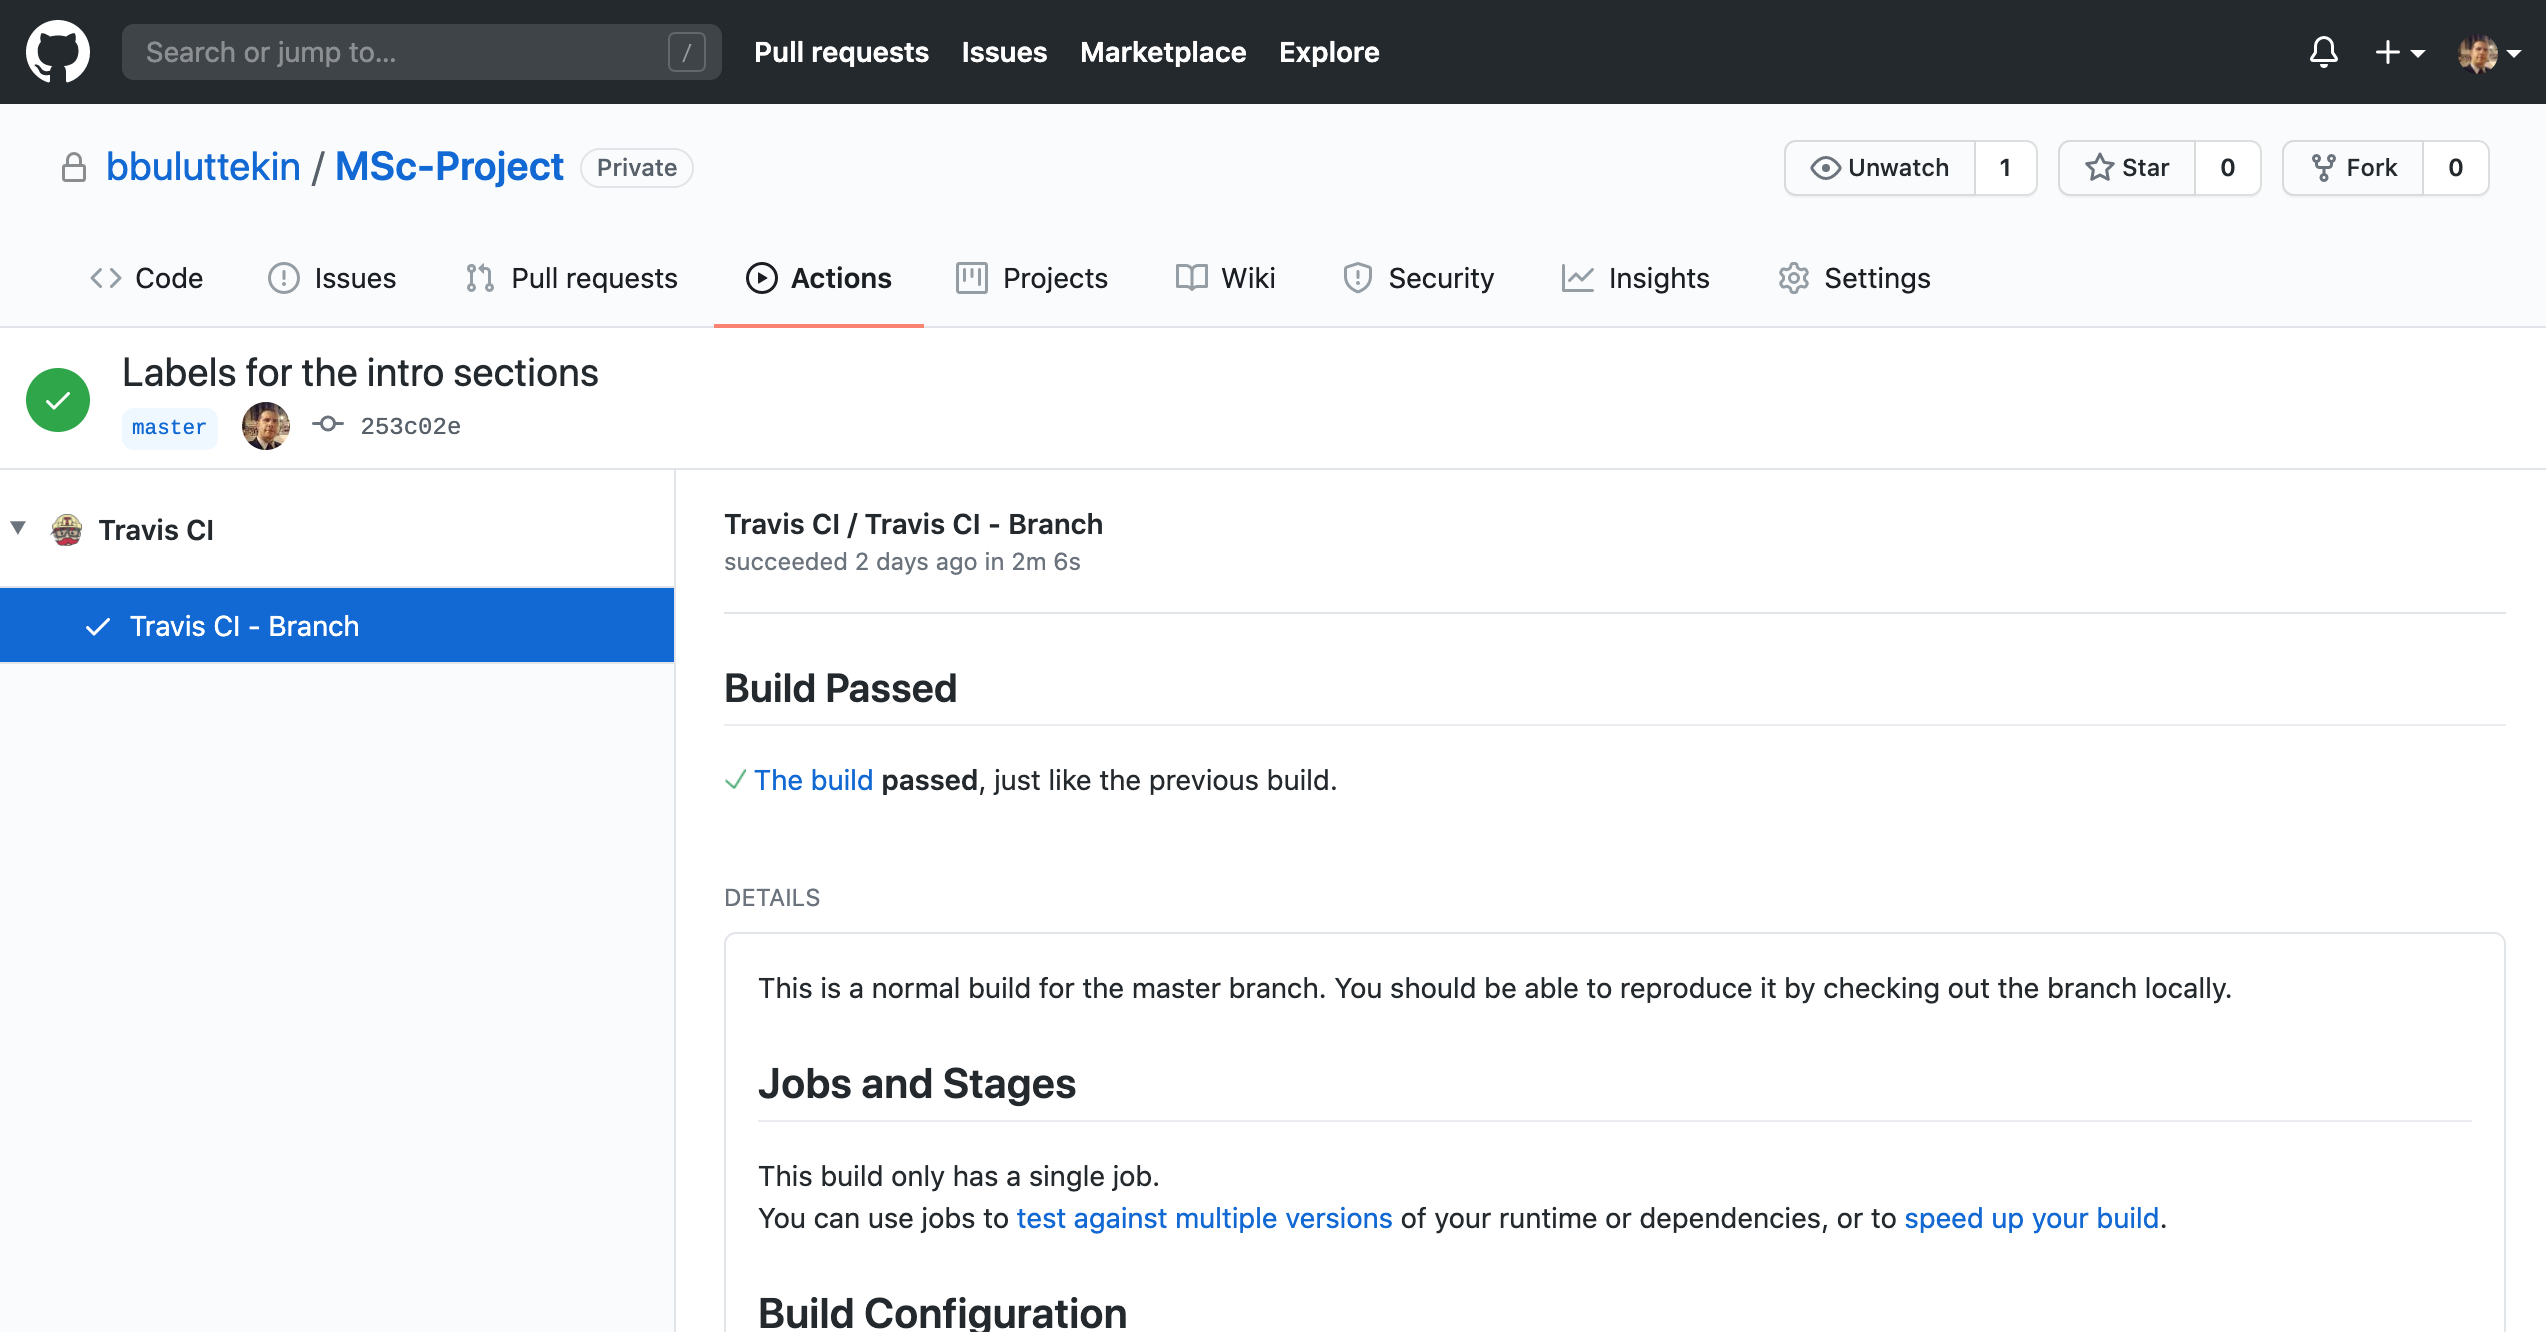
\includegraphics[width=\textwidth]{img/cigithub.png}
    \caption{CI feedback received from Travis.}
    \label{fig:cigithub}
\end{figure}
 


\section{Project specification and design} \label{sec:projectlayout}
This project I aimed to keep code and reporting together to provide easy reproduction. Codebase design to be extendable and modular. Therefore, I assign a sub-folder for all the project-specific code under the name \emph{src}. Having a module in the same directory level with the other components allows the ability to use the code in notebook experiment as well as in the tests in the CI integration.
Both project proposal and report developed using the LaTeX typesetting system and documents kept in the version controlling to allow easy changes and rolling back to best version.

Overall project design such as folders and library interactions.

\dirtree{%
.1 .
.2 Proposal.
.3 Proposal files.
.2 Report.
.3 chapters.
.4 Chapter files.
.3 img.
.4 Images.
.3 Main project latex files.
.2 scripts.
.3 Utility scripts.
.2 notebooks.
.3 Experiment notebooks.
.2 src.
.3 Python library files.
.2 tests.
.3 Test files.
.2 .gitignore.
.2 .travis.
.2 README.md.
.2 requirements.txt.
}

\section{Reproducibility Guidance} \label{sec:reproducibility}
Reproducibility is a fundamental 

As a scientific project, it is very important that anyone can reproduce the experiments and findings in this project to verify the conclusions reached are accurate. \cite{dataset}


to reproduce the experiments and findings in this project to verify the conclusions reached are accurate.

Parts to consider before reproducing.
Repo is not public
Most runs carried out in colab 
notebooks should be positioned in same level as the src library
running shell utility files requires kaggle api key


\clearpage